\chapter{One Random Variable}


\section{The Cumulative Distribution Function}

\bit
	\item The \emph{cumulative distribution function}
	has the advantage that it is
	\emph{not limited} to discrete random variables
	and applies to all types of random variables.

	\item

	\begin{defn}
	Consider a random experiment with sample space \sspace\
	and event class \evcl.
	A random variable \X\ is a function from the sample space \sspace\
	to $\reals$ with the property that the set
	$A_b = \set{\zeta}{X(\zeta)\leq b}$
	is in \evcl\ for every $b$ in $\reals$.
	\end{defn}

	\item The \emph{cumulative distribution function} (CDF)
	of a random variable \X\ is defined as the probability of the event
	$\{X\leq x\}$:
	\beql{eq-def-cdf}
		\cdfxk{x} = \pr{X\leq x}
	\eeql
	for $x\in\reals$.
	\begin{itemize}
		\item
		It is the probability that the random variable \X\
		takes on a value in the set $(-\infty,x]$.
		In terms of the underlying sample space,
		the CDF is the probability of the event
		$\set{\zeta}{X(\zeta) \leq x}$.
		\item
		\emph{\cdfxk{x}\ is a function of the variable $x$.}
	\end{itemize}


	\item
	The events of interest when dealing with numbers are intervals
	of the real line, and their complements, unions, and intersections.
	We show below that the probabilities of all of these events
	can be expressed in terms of the CDF.

	\item \lgexam{4.1}{Three Coin Tosses}
	\figurename~\ref{fig-cdfpdf1}
	shows the CDF and probability density function (PDF)
	of the \binomrv\ with $n=3$ and $p=1/2$.

	\begin{figure}\begin{center}
	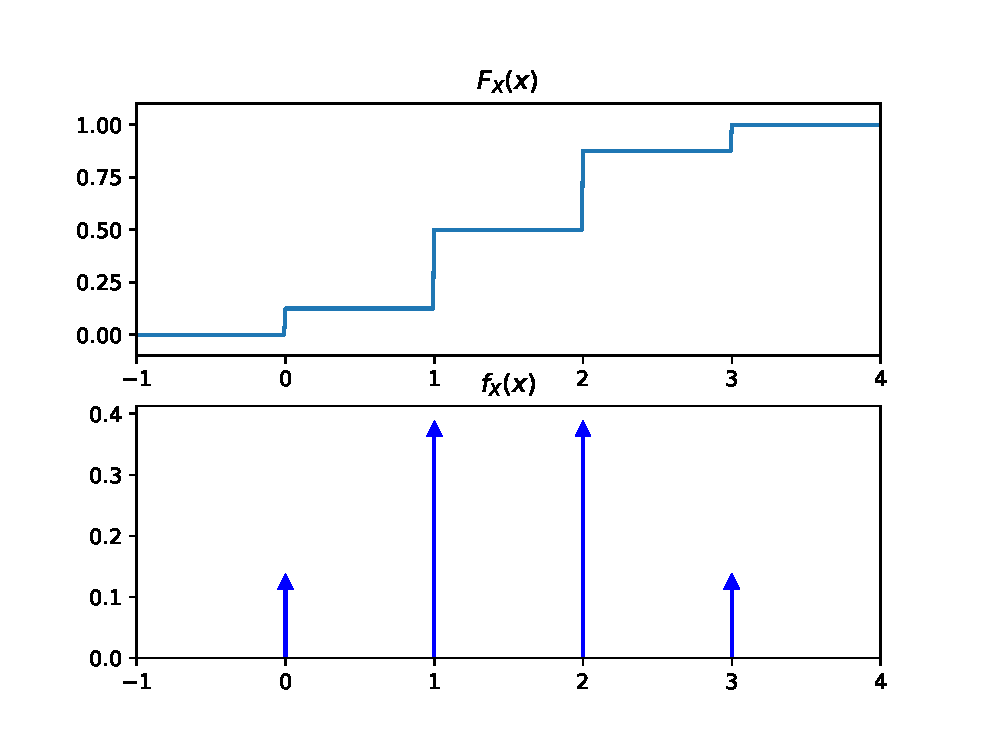
\includegraphics[width=.7\linewidth]{figures/cdfpdf1}
	\caption{The CDF and PDF of the \binomrv\ with $n=3$ and $p=1/2$.}
	\label{fig-cdfpdf1}
	\end{center}\end{figure}

	\begin{itemize}
		\item The CDF is continuous from the right
		and equal to $1/2$ at the point $x = 1$.
		\[
			\lim_{x\to 1+0} \cdfxk{x} = 1/2,\
			\lim_{x\to 1-0} \cdfxk{x} = 1/8.
		\]

		\item
		Indeed, we note the magnitude of the jump
		at the point $x = 1$ is equal to
		$\pr{X = 1} = 1/2 - 1/8 = 3/8$.
	\end{itemize}


	\item \lgexam{4.2}{Uniform Random Variable in the Unit Interval}
	\figurename~\ref{fig-unif-ff}
	shows the CDF and PDF
	of the \unifrv\ with support $[0,1]$.

	\begin{figure}\begin{center}
	\includegraphics[width=.7\linewidth]{figures/unif_ff}
	\caption{The CDF and PDF of the \unifrv\ with support $[0,1]$.}
	\label{fig-unif-ff}
	\end{center}\end{figure}

	\begin{itemize}
		\item No discontinuity in the CDF
		\item The derivative of CDF coincides with the PDF (except two points, $x=0$ and $x=1$).
	\end{itemize}


	\item Basic properties of the CDF:
	The axioms of probability and their corollaries
	imply that the CDF has the following properties:

	\renewcommand{\labelenumi}{(\roman{enumi})}
	\renewcommand{\theenumi}{(\roman{enumi})}
	\begin{enumerate}
		\item \label{cdf-bp-1}
		$0\leq \cdfxk{x} \leq 1$.

		\item \label{cdf-bp-2}
		$\lim_{x\to\infty} \cdfxk{x} = 1$.

		\item \label{cdf-bp-3}
		$\lim_{x\to-\infty} \cdfxk{x} = 0$.

		\item \label{cdf-bp-4}
		\cdfxk{x}\ is a nondecreasing function of $x$,
		that is, if $a < b$, then $\cdfxk{a} \leq \cdfxk{b}$.

		\item \label{cdf-bp-5}
		\cdfxk{x}\ is continuous from the right, \ie,
		\[
			\cdfxk{x} = \lim_{h\to+0} \cdfxk{x+h} = \cdfxk{x^+}.
		\]

		\item \label{cdf-bp-6}
		$\pr{a< X\leq b} = \cdfxk{b} - \cdfxk{a}$.

		\item \label{cdf-bp-7}
		$\pr{X=b} = \cdfxk{b} - \cdfxk{b^-}$.

		\item \label{cdf-bp-8}
		$\pr{X>x} = 1- \cdfxk{x}$.

	\end{enumerate}

	\begin{itemize}

		\item
		The first five properties confirm that,
		in general, the CDF is
		a nondecreasing function that grows from $0$ to $1$
		as $x$ increases from $-\infty$ to $\infty$.

		\item
		Property \ref{cdf-bp-7}
		states that the probability that $X = b$
		is given by the magnitude of the jump of the cdf at the point $b$.
		This implies that if the CDF is continuous at a point $b$,
		then $\pr{X = b} = 0$.

		\item Properties \ref{cdf-bp-6} and \ref{cdf-bp-7}
		can be combined to compute the probabilities of other types
		of intervals.
		For example,
		since $\{a\leq X\leq b\} = \{X=a\} \cup \{a<X\leq b\}$,
		then
		\[
			\pr{a\leq X\leq b}
			= \pr{X=a} + \pr{a<X\leq b}
			= \cdfxk{a}-\cdfxk{a^-}
			+ \cdfxk{b} - \cdfxk{a}
			= \cdfxk{b} -\cdfxk{a^-}.
		\]

		\item While intuitively clear,
		\emph{
		properties
		\ref{cdf-bp-2},
		\ref{cdf-bp-3},
		\ref{cdf-bp-5},
		and
		\ref{cdf-bp-7}
		require more advanced limiting arguments.}


	\end{itemize}

	\renewcommand{\labelenumi}{\arabic{enumi}.}
	\renewcommand{\theenumi}{\arabic{enumi}.}


\eit

\subsection{The Three Types of Random Variables}

\bit
	\item
	A \emph{discrete random variables}
	has a CDF that is a right-continuous,
	staircase function of $x$,
	with jumps at a countable set of points.
	The CDF \cdfxk{x}\ of a discrete random variable
	is the sum of the probabilities of the outcomes
	less than $x$
	and \emph{can be written as the weighted sum of unit step functions}
	\beql{eq-cdf-disc-sum-unit}
		\cdfxk{x} = \sum_{x_k\leq x} \pmfxk{x_k}
		= \sum_k \pmfxk{x_k} u(x-x_k)
	\eeql
	where the PMF $\pmfxk{x_k}$ gives the magnitude of the jumps in the CDF.

	\item A \emph{continuous random variable}
	is defined as a random variable whose \emph{CDF \cdfxk{x}\
	is continuous everywhere,
	and which, in addition, is sufficiently smooth}
	that it can be written as an \emph{integral of some nonnegative function $f(x)$}:
	\beql{eq-cdf-as-int-pdf}
		\cdfxk{x} = \int_{-\infty}^x \pdfxk{x} \dx.
	\eeql

	\begin{itemize}
		\item The continuity of the CDF and property \ref{cdf-bp-7} implies
		that continuous random variables have
		\emph{$\pr{X = x} = 0$ for all $x$}.
		\emph{Every possible outcome has probability zero!}


		\item  We calculate probabilities as
		integrals of ``probability densities'' over
		intervals of the real line,
		\ie,
		\[
			\pr{a\leq X\leq b} = \int_a^b \pdfxk{x}.
		\]
	\end{itemize}


	\item A \emph{random variable of mixed type}
	is a random variable with a CDF that has jumps
	on a countable set of points,
	but that also increases continuously over
	\emph{at least one interval} of values of $x$.
	\begin{itemize}
		\item The CDF for these random variables has
		the form
		\[
			\cdfxk{x} = p \cdfk{X_1}{x} + (1-p) \cdfk{X_2}{x}
		\]
		where $0 < p < 1$,
		and \cdfk{X_1}{x}\ is the CDF of a discrete random variable, $X_1$,
		and \cdfk{X_2}{x}\ is the CDF of a continuous random variable, $X_2$.
	\end{itemize}
\eit

\subsection{Fine Point: Limiting properties of CDF \optional}

\bit
	\item Properties
	\ref{cdf-bp-2},
	\ref{cdf-bp-3},
	\ref{cdf-bp-5},
	and
	\ref{cdf-bp-7}
	require the continuity property of the probability function
	discussed in \S\ref{sec:fine-points-2}.

	\item For {property \ref{cdf-bp-2}},
	we consider the sequence of events $\{X \leq n\}$
	which increases to include all of the sample space \sspace\
	as $n$ approaches $\infty$,
	that is,
	all outcomes lead to a value of \X\ less than infinity. 
	The continuity property of the probability function
	(\corollaryname~\ref{coro-cont-prob-fcn}) implies that:
	\[
		\limninfty \cdfxk{n} =
		\limninfty \pr{X\leq n} =
		\bpr{ \limninfty \{X\leq n\} } =
		\pr{\sspace} =
		1.
	\]

	\item For {property \ref{cdf-bp-3}},
	we take the sequence $\{X \leq n\}$
	which decreases to the empty set $\emptyset$,
	that is, no outcome leads to a value of \X\ less than $-\infty$:
	\[
		\limninfty \cdfxk{-n} =
		\limninfty \pr{X\leq -n} =
		\bpr{ \limninfty \{X\leq -n\} } =
		\pr{\emptyset} =
		0.
	\]

	\item For property \ref{cdf-bp-5},
	we take the sequence of events $\{X\leq b + 1/n\}$
	which decreases to $\{X\leq b\}$
	from the right:
	\begin{eqnarray*}
		\limninfty \cdfxk{b+1/n} &=& \limninfty \pr{X\leq b + 1/n}
		\\&=&
		\bpr{\limninfty \{X \leq b + 1/n\}} =
		\pr{\{X\leq b\}} =
		\cdfxk{b}.
	\end{eqnarray*}

	\item For property \ref{cdf-bp-7},
	we take the sequence of events,
	$\{b-1/n< X \leq b\}$
	which decreases to $\{b\}$
	from the left:
	\begin{eqnarray*}
		\limninfty (\cdfxk{b} - \cdfxk{b-1/n})
		&=& \limninfty \pr{b-1/n< X\leq b }
		\\&=&
		\bpr{\limninfty \{b-1/n< X\leq b \}}
		=
		\pr{X=b}.
	\end{eqnarray*}
\eit



\section{The Probability Density Function}
\bit
	\item The probability density function (PDF) of \X,
	if it exists, is defined as the derivative of \cdfxk{x}:
	\beql{eq-def-pdf}
		\pdfxk{x} = \frac{d\cdfxk{x}}{dx}.
	\eeql

	\item The PDF is an alternative,
	and more useful,
	way of specifying the information
	contained in the cumulative distribution function.

	\item The PDF represents the ``density'' of probability
	at the point $x$ in the following sense:
	The probability that \X\ is in a small interval
	in the vicinity of $x$,
	\ie,
	\[
		\pr{x< X\leq x+h}
		= \cdfxk{x+h} - \cdfxk{x}
		= \frac{\cdfxk{x+h} - \cdfxk{x}}{h} h
		\simeq  \pdfxk{x} h
	\]
	for very small $h$.

	\item Properties of the PMF:

	\renewcommand{\labelenumi}{(\roman{enumi})}
	\renewcommand{\theenumi}{(\roman{enumi})}
	\begin{enumerate}
		\item Since \cdfxk{x} is nondecreasing,
		\beql{eq-pdf-bp-1}
			\pdfxk{x} \geq 0
		\eeql

		\item (Almost) by definition,
		\beql{eq-pdf-bp-2}
			\pr{a\leq X\leq b} = \int_a^b \pdfxk{x} \dx.
		\eeql
		\begin{itemize}
			\item The probability of an interval is
			therefore the area under \pdfxk{x}\ in that interval,
			as shown in \figurename~\ref{fig-lg-4-4}.
			
			\begin{figure}\begin{center}
			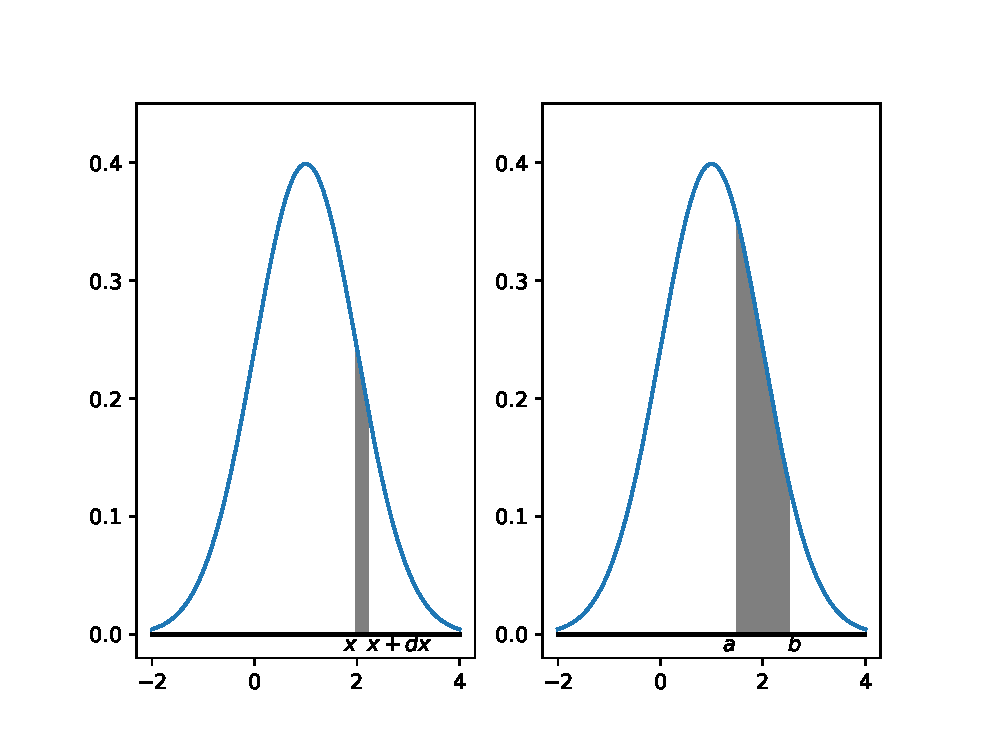
\includegraphics[width=.8\linewidth]{figures/fig4_4}
			\caption{
			(left) The PDF specifies the probability of intervals of
			infinitesimal width.
			(right) The probability of an interval $[a,b]$
			is the area under the PDF in the interval.
			}
			\label{fig-lg-4-4}
			\end{center}\end{figure}
		\end{itemize}

		\item The CDF of \X\ can be obtained by integrating the PDF:
		\beql{eq-pdf-bp-3}
			\cdfxk{x} = \int_{-\infty}^x \pdfxk{t}  \dt.
		\eeql
		\begin{itemize}
			\item Thus the PDF
			completely specifies the behavior of continuous random variables.
		\end{itemize}

		\item By letting $x$ tend to infinity in (\ref{eq-pdf-bp-3}),
		we obtain a \emph{normalization} condition for the PDF:
		\beql{eq-pdf-bp-4}
			1 = \int_{-\infty}^\infty \pdfxk{x} \dx.
		\eeql

		
	\end{enumerate}
	\renewcommand{\labelenumi}{\arabic{enumi}.}
	\renewcommand{\theenumi}{\arabic{enumi}.}

	\item
	A valid PDF can be formed from any nonnegative,
	piecewise continuous function $g(x)$ that has a finite integral:
	\beql{eq-nonneg-fcn}
		\intinftoinf g(x) \dx = c < \infty.
	\eeql


	\item \lgexam{4.6}{Uniform Random Variable}
	The PDF of the \unifrv\ is given by
	\[
		\pdfxk{x} = \left\{\begin{array}{ll}
		1/(b-a)	&a \leq x\leq b
		\\0	&\mbox{otherwise}
		\end{array}
		\right.
	\]
	and the CDF is given by
	\[
		\cdfxk{x} = \left\{\begin{array}{ll}
		0	& x < a
		\\(x-a)/(b-a)	&a \leq x\leq b
		\\1	&x > b
		\end{array}
		\right.
	\]
	as in \figurename~\ref{fig-unif-ff}.

	\item \lgexam{4.7}{Exponential Random Variable}
	The PDF and CDF are given by
	\[
		\pdfxk{x} = \ld e^{-\ld x} u(x)
	\]
	and
	\[
		\pdfxk{x} = (1- e^{-\ld x}) u(x)
	\]
	where $u(x)$ is the unit step function:
	\[
		u(x) = \left\{\begin{array}{ll}
			1	&\mif x \geq 0
			\\0	&\mif x < 0
		\end{array}
		\right.
	\]
	
\eit


\subsection{PDF of Discrete Random Variable}

\bit
	\item
	The derivative of the CDF does \emph{not} exist at points
	where the CDF is \emph{not continuous}.
	Thus the notion of PDF as defined by
	(\ref{eq-def-pdf})
	does not apply to discrete random variables
	at the points where the CDF is discontinuous.

	\item We can generalize the definition of the probability density function
	by noting the relation between the \emph{unit step function}
	and the \emph{delta function}.


	\item 
	The \emph{unit step function} is defined as
	\beql{eq-def-unit}
		u(x) = \left\{\begin{array}{ll}
			1	&\mif x \geq 0
			\\0	&\mif x < 0.
		\end{array}
		\right.
	\eeql

	\item The \emph{(Dirac) \delfcn} $\delta(x)$
	is related to the \unitfcn\ bu the following equation:
	\beql{eq-def-delta}
		u(x) = \int_{-\infty} ^ x \delta(t) \dt
	\eeql

	\item The translated \unitfcn\ is then:
	\beql{eq-trans-delta}
		u(x-x_0) = \intinfto{x-x_0} \delta(t) \dt
		= \intinfto{x} \delta(t-x_0) \dt
	\eeql

	\item Substituting (\ref{eq-trans-delta}) into (\ref{eq-cdf-disc-sum-unit})
	yields
	\begin{eqnarray*}
		\cdfxk{x}
		=  \sum_k \pmfxk{x_k} u(x-\xk)
		=  \sum_k \pmfxk{x_k} \intinfto{x} \delta(t-\xk) \dt
		=  \intinfto{x} \sum_k \pmfxk{x_k} \delta(t-\xk) \dt
	\end{eqnarray*}


	\item This suggests that we define the PDF for a discrete random variable
	by
	\beql{eq-pdf-disc-sum-delta}
		\pdfxk{x} = \frac{d}{dx} \cdfxk{x}
		=  \sum_k \pmfxk{x_k} \delta(t-\xk) \dt
	\eeql
	\begin{itemize}
		\item
		Thus the generalized definition of PDF places
		a delta function of weight \pr{X = \xk}\ at the points \xk\
		where the CDF is discontinuous.
	\end{itemize}

	\item \emph{Please read the parts explaining the delta function}!
	\begin{itemize}
		\item The Dirac \delfcn\ has the following property:
		\beql{eq-del-prop-1}
			\intinftoinf g(t) \delta(t-x) \dt = g(x).
		\eeql
	\end{itemize}

	\item The \emph{PDF of a random variable of mixed type}
	will also contain delta functions at the points where its CDF is not continuous.

	\item \lgexam{4.9}{}
	The \binomrv\ with $n=3$ and $p=1/2$.
	The CDF is
	\[
		\cdfxk{x} =
		\frac{1}{8} u(x)
		+\frac{3}{8} u(x-1)
		+\frac{3}{8} u(x-2)
		+\frac{1}{8} u(x-3)
	\]
	and the PDF is
	\[
		\pdfxk{x} =
		\frac{1}{8} \delta(x)
		+\frac{3}{8} \delta(x-1)
		+\frac{3}{8} \delta(x-2)
		+\frac{1}{8} \delta(x-3).
	\]
\eit

\subsection{Conditional CDFs and PDFs}

\bit
	\item The \emph{conditional CDF} of \X\ given the event $C$ is defined by
	\beql{eq-def-cond-cdf}
		\ccdfxk{x}{C} = 
		\frac{\cpr{\{X\leq x\}} \cap C }{\pr{C}}
	\eeql
	where $\pr{C} > 0$.

	\begin{itemize}
		\item easy to show that \ccdfxk{x}{C}\ satisfies
		all the properties of a CDF.
		(See Problem 4.29.) The conditional pdf of X given C is then defined by
	\end{itemize}


	\item The \emph{conditional PDF} of \X\ given the event $C$ is defined by
	\beql{eq-def-cond-pdf}
		\cpdfxk{x}{C} = 
		\frac{d}{dx} \ccdfxk{x}{C}
	\eeql

	\item Suppose that we have a partition of the sample space \sspace\
	into the union of disjoint events $B_1$, $B_2$, \ldots, $B_n$.
	Let \ccdfxk{x}{B_i}\ be the conditional CDF of \X\ given event $B_i$.
	The \emph{theorem on total probability}
	allows us to find the CDF of \X\ in terms of the conditional CDFs:
	\beql{eq-theorem-total-prob-cdf}
		\ccdfxk{x}
		= \pr{X\leq x}
		= \sumiton \cpr{X\leq x}{B_i} \pr{B_i}
		= \sumiton \ccdfxk{x}{B_i} \pr{B_i}
	\eeql

	\begin{itemize}
		\item The PDF is obtained by differentiation:
		\beql{eq-theorem-total-prob-pdf}
			\pdfxk{x} =  \ddx \cdfxk{x}
			= \sumiton \cpdfxk{x}{B_i} \pr{B_i}.
		\eeql
	\end{itemize}


	\item \lgexam{4.11}{A binary transmission system}
	A binary transmission system sends a ``0'' bit by transmitting
	a $-v$ voltage signal,
	and a ``1'' bit by transmitting a $+v$.
	The received signal is corrupted by Gaussian noise and given by:
	\[
		Y = X + N
	\]
	where \X\ is the transmitted signal,
	and $N$ is a noise voltage with PDF \pdfk{N}{x}.
	Assume that $\pr{``1''} = p = 1 = \pr{``0''}$
	and that $N$ is \gaussrv\ with $0$ and $\sigma$ as its mean and standard deviation,
	\ie,
	\[
		\pdfk{N}{x} =
		{\frac{1}{\sqrt{2\pi} {\sigma}} e^{-x^2/2{\sigma}^2} }
	\]

	Find the PDF of $Y$.

	\begin{itemize}
		\item The PDF is
		\[
			\pdfk{Y}{x}
			= \cpdfk{Y}{x}{B_0} \pr{B_0}
			+ \cpdfk{Y}{x}{B_1} \pr{B_1}
			=
			\gausspdf{x}{+v}{\sigma} (1-p)
			+ \gausspdf{x}{-v}{\sigma} p.
		\]

		\item 
		\lgfig{4.5}\ shows the two conditional PDFs.
		The transmitted signal \X\ shifts the center of mass of the Gaussian PDF.
	\end{itemize}

\eit


\section{The Expected Value of \X}

\bit
	\item The \emph{expected value} or \emph{mean} of a random variable \X\
	is defined by
	\beql{eq-def-expect-cont}
		\Exp{X} = \intinftoinf x\pdfxk{x} \dx.
	\eeql
	The expected value \Exp{X}\ is defined if the above integral converges absolutely,
	that is,
	\beql{eq-def-expect-cont-abs-conv}
		\Exp{X} = \intinftoinf |x| \pdfxk{x} \dx.
	\eeql

	\item If we view \pdfxk{x}\
	as the \emph{distribution of mass on the real line},
	then \Exp{X}\ represents the \emph{center of mass} of this distribution.


	\item The definition in (\ref{eq-def-expect-cont})
	is applicable if we express the PDF of a discrete random variable using \delfcn s:
	\[
		\Exp{X}
		= \intinftoinf x \sum_k \pmfxk{\xk} \delta(x-\xk) \dx
		= \sum_k \pmfxk{\xk} \intinftoinf x \delta(x-\xk) \dx
	\]
	where (\ref{eq-del-prop-1}) is used for the last equality.


	\item \lgexam{4.12}{Mean of a Uniform Random Variable}

	The PDF of the \unifrv\ is
	\[
		\pdfxk{x} = \left\{\begin{array}{ll}
		1/(b-a)	&a \leq x\leq b
		\\0	&\mbox{otherwise},
		\end{array}
		\right.
	\]
	hence
	\[
		\Exp{X} = \int_a^b x \frac{1}{b-a} \dx
		= \frac{1}{b-a} \cdot \frac{1}{2} (b-a)^2
		= \frac{a+b}{2}.
	\]

	\item If $\pdfxk{m-x} = \pdfxk{m+x}$ for all $x\in\reals$,
	then $\Exp{X} = m$ since
	\[
		0 = \intinftoinf (m-x) \pdfxk{x} \dx
		= \intinftoinf m \pdfxk{x} \dx
		- \intinftoinf x \pdfxk{x} \dx
		= m - \Exp{X}.
	\]


	\item \lgexam{4.13}{Mean of a Gaussian Random Variable}

	The PDF of a Gaussian random variable $e^{-(x-m)^2/\sigma^2}/\sqrt{2\pi}\sigma$
	is symmetric about the point $x = m$,
	hence $\Exp{X} = m$.

	\item Aother formulas for \Exp{X}:
	\begin{itemize}
		\item For nonnegative continuous \randvar s:
		\beql{eq-int-exp-cont}
			\Exp{X} = \int_0^\infty (1-\cdfxk{x}) \dx
		\eeql

		\item For nonnegative integer-valued \randvar s:
		\beql{eq-int-exp-disc}
			\Exp{X} = \sumkztoi \pr{X>k}
		\eeql
	\end{itemize}


	\item \lgexam{4.14}{Mean of Exponential Random Variable}

	\[
		\Exp{X}
		= \intinftoinf  \ld e^{-\ld x} \dx
	\]


	
\eit

\section{Important Continuous Random Variables}

\section{Functions of a Random Variable}

\section{The Markov and Chebyshev Inequalities}

\section{Transform Methods}

\section{Basic Reliability Calculations}

\section{Computer Methods for Generating Random Variables}

\section{Entropy \optional}

